\documentclass{beamer}
\usepackage{stile_presentazione}

\title[]{Confronto di tecniche di embeddings in ambienti\\ di Graph Data Science distribuiti: un caso \\di studio in ambito biomedico}
\author[Sandi Russo]{Sandi Russo}
\date{}


\begin{document}


% frontespizio
\iniziofrontespizio
\begin{frame}[plain]
  \begin{tikzpicture}[remember picture, overlay]
    \node[anchor=north] at ([yshift=-0.8cm]current page.north)
      {
\includegraphics[height=1.8cm]{figures/logo_unime.png}};
\node[anchor=center, text width=12cm, align=center] at ([yshift=0.5cm]current page.center)
  {{\sloppy\large\textcolor{white}{\textbf{\inserttitle}}}};
    \node[anchor=south west, align=left] at ([xshift=0.8cm, yshift=1.2cm]current page.south west)
      {\footnotesize\textcolor{Gray}{Candidato}\\[2pt]\textcolor{white}{\textbf{Sandi Russo}}};
    \node[anchor=south east, align=right] at ([xshift=-0.8cm, yshift=1.2cm]current page.south east)
      {\footnotesize\textcolor{Gray}{Relatore}\\[2pt]\textcolor{white}{\textbf{Prof. Antonio Celesti}}};
  \end{tikzpicture}
\end{frame}
\finefrontespizio



% prima slide
\begin{frame}{Il modello Property Graph}

  Un database a grafo archivia e rappresenta l'informazione\\
  attraverso nodi e relazioni. La sua massima espressione è \hl{Neo4j}.

  \vspace{0.5em}

  \begin{columns}
    \column{0.45\textwidth}
      \begin{itemize}
        \item \textbf{Nodo}: rappresenta un'entità nel grafo
        \item \textbf{Relazione}: connette i nodi con tipo e direzione
        \item \textbf{Proprietà}: coppie chiave-valore su nodi e relazioni
        \item \textbf{Label}: classificano semanticamente i nodi
      \end{itemize}

    \column{0.55\textwidth}
      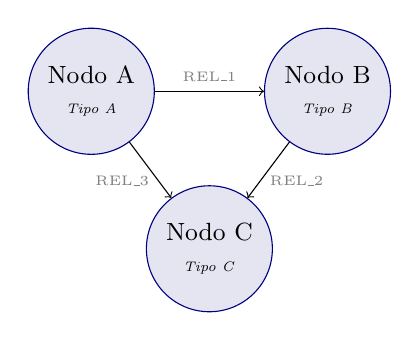
\begin{tikzpicture}[
        node/.style={circle, draw=Navy, fill=Navy!10, minimum width=1.6cm,
                     minimum height=1.2cm, font=\small, align=center},
        every edge/.style={draw, ->, thick, Navy},
        prop/.style={font=\tiny, color=Gray}
      ]
        \node[node] (A) at (0,0) {Nodo A\\\textit{\tiny Tipo A}};
        \node[node] (B) at (3,0) {Nodo B\\\textit{\tiny Tipo B}};
        \node[node] (C) at (1.5,-2) {Nodo C\\\textit{\tiny Tipo C}};
        \draw[->] (A) -- node[above, prop] {REL\_1} (B);
        \draw[->] (B) -- node[pos=0.7, right, prop] {REL\_2} (C);
        \draw[->] (A) -- node[pos=0.7, left, prop] {REL\_3} (C);
      \end{tikzpicture}
  \end{columns}

\end{frame}



% seconda slide
\begin{frame}{Graph Data Science}

    La GDS combina algoritmi su grafi e tecniche di \hl{Machine Learning} per estrarre conoscenza predittiva dalla struttura topologica di reti complesse, superando i limiti dei database relazionali.

  \vspace{0.5em}

  \begin{columns}[t]
    \column{0.33\textwidth}
      \textcolor{Cyan}{\textbf{Queries}}\\[4pt]
      \small Esplorare il grafo per trovare schemi e pattern noti.

    \column{0.33\textwidth}
      \textcolor{Cyan}{\textbf{Machine Learning}}\\[4pt]
      \small Fare previsioni su connessioni non ancora documentate.

    \column{0.33\textwidth}
      \textcolor{Cyan}{\textbf{Visualization}}\\[4pt]
      \small Visualizzare e analizzare i risultati degli algoritmi.
  \end{columns}

  \vspace{0.8em}

  \begin{center}
  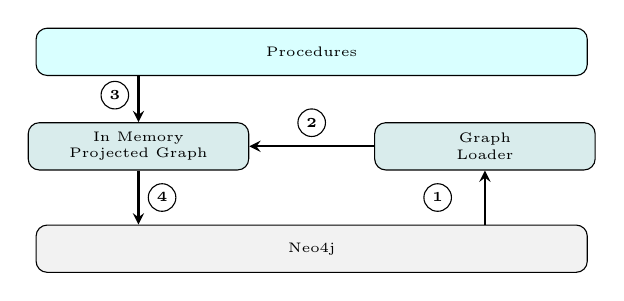
\begin{tikzpicture}[
    box/.style={rectangle, draw, rounded corners, minimum height=0.6cm,
                font=\tiny, align=center},
    wide_box/.style={box, minimum width=7cm},
    node_box/.style={box, minimum width=2.8cm, minimum height=0.6cm},
    arrow/.style={->, thick, >=stealth},
    number/.style={circle, draw, fill=white, inner sep=1pt,
                   minimum size=0.35cm, font=\tiny\bfseries}
  ]
    \node[wide_box, fill=Cyan!15]  (proc)   at (0, 3) {Procedures};
    \node[wide_box, fill=gray!10]  (neo4j)  at (0, 0.5)   {Neo4j};
    \node[node_box, fill=teal!15]  (impg)   at (-2.2, 1.8) {In Memory\\Projected Graph};
    \node[node_box, fill=teal!15]  (loader) at (2.2, 1.8)  {Graph\\Loader};

    \draw[arrow] (neo4j.north -| loader.south) -- (loader.south);
    \node[number] at (1.6, 1.15) {1};
    \draw[arrow] (loader.west) -- (impg.east);
    \node[number] at (0, 2.1) {2};
    \draw[arrow] (proc.south -| impg.north) -- (impg.north);
    \node[number] at (-2.5, 2.45) {3};
    \draw[arrow] (impg.south) -- (neo4j.north -| impg.south);
    \node[number] at (-1.9, 1.15) {4};
  \end{tikzpicture}
  \end{center}

\end{frame}



% terza slide
\begin{frame}{Il problema: drug repurposing}

  Identificare nuove applicazioni terapeutiche per farmaci già esistenti
  è più rapido ed economico della ricerca tradizionale, ma richiede
  l'analisi di reti biologiche di \hl{scala massiva}.

  \vspace{0.8em}

  \begin{columns}[t]
    \column{0.48\textwidth}
      \textcolor{Cyan}{\textbf{Lacuna algoritmica}}\\[4pt]
      \small La maggior parte dei lavori valuta i modelli su dataset
      omogenei o di dimensioni contenute. Manca un confronto strutturato
      su KG biomedici reali di scala massiva.

    \column{0.48\textwidth}
      \textcolor{Cyan}{\textbf{Lacuna infrastrutturale}}\\[4pt]
      \small La letteratura assume il grafo già in memoria, ignorando
      la fase critica di estrazione da un Graph DBMS distribuito verso
      il framework di apprendimento.

  \end{columns}

  \vspace{0.8em}

  \begin{center}
    \small\textcolor{Gray}{Obiettivo: una valutazione \textbf{end-to-end}
    che colleghi infrastruttura distribuita e qualità predittiva degli embedding.}
  \end{center}

\end{frame}



% quarta slide
\begin{frame}{Il dataset: PharMeBiNet V3}

  Un knowledge graph biomedico open-source che integra oltre
  quaranta sorgenti farmacologiche, genomiche e cliniche in
  un'unica struttura a grafo \hl{eterogeneo}.

  \vspace{1em}

  \begin{columns}[c]
    \column{0.33\textwidth}
      \kpi{8M}{nodi su 80 label distinte}

    \column{0.33\textwidth}
      \kpi{53M}{relazioni di 410 tipi}

    \column{0.33\textwidth}
      \kpi{123.361}{archi Chemical$\to$Disease}
  \end{columns}

  \vspace{1em}

  \begin{center}
    \small\textcolor{Gray}{Scelto per scala, eterogeneità strutturale
    e rilevanza applicativa nel contesto del drug repurposing.}
  \end{center}

\end{frame}



% quinta slide
\begin{frame}{I tre paradigmi a confronto}

  La scelta degli algoritmi esplora tre filosofie architetturali
  distinte, permettendo di isolare l'impatto di ciascuna
  sulla qualità degli \hl{embedding} prodotti.

  \vspace{0.8em}

  \begin{center}
  \begin{tabular}{lccc}
    \toprule
    & \textbf{GraphSAGE} & \textbf{HashGNN} & \textbf{TransE} \\
    \midrule
    Paradigma
      & Induttivo & Induttivo & Trasduttivo \\[4pt]
    Spazio embedding
      & Omogeneo & Eterogeneo & Geometrico \\[4pt]
    Aggregazione vicinato
      & \textcolor{Cyan}{Sì} & \textcolor{Cyan}{Sì} & \textcolor{Orange}{No} \\[4pt]
    Generalizza a nodi nuovi
      & \textcolor{Cyan}{Sì} & \textcolor{Cyan}{Sì} & \textcolor{Orange}{No} \\[4pt]
    Gestione eterogeneità
      & \textcolor{Orange}{No} & \textcolor{Cyan}{Sì} & \textcolor{Orange}{No} \\
    \bottomrule
  \end{tabular}
  \end{center}
\end{frame}



% settima slide
\begin{frame}{GraphSAGE}

  Apprende una \hl{funzione di aggregazione} generalizzabile
  invece di un vettore fisso per nodo, generalizzando a entità
  non osservate durante il training.

  \vspace{0.5em}

  \begin{center}
  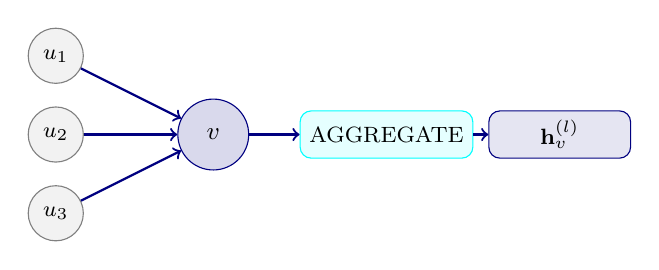
\begin{tikzpicture}[
    mainnode/.style={circle, draw=Navy, fill=Navy!15,
                     minimum size=0.9cm, font=\small},
    neighnode/.style={circle, draw=Gray, fill=Gray!10,
                      minimum size=0.7cm, font=\footnotesize},
    aggbox/.style={rectangle, draw=Cyan, rounded corners,
                   fill=Cyan!10, minimum width=1.8cm,
                   minimum height=0.6cm, font=\footnotesize},
    outbox/.style={rectangle, draw=Navy, rounded corners,
                   fill=Navy!10, minimum width=1.8cm,
                   minimum height=0.6cm, font=\footnotesize},
    arrow/.style={->, thick, Navy}
  ]
    \node[neighnode] (n1) at (-3, 1.0)  {$u_1$};
    \node[neighnode] (n2) at (-3, 0)    {$u_2$};
    \node[neighnode] (n3) at (-3, -1.0) {$u_3$};
    \node[mainnode]  (v)  at (-1, 0)    {$v$};

    \draw[arrow] (n1) -- (v);
    \draw[arrow] (n2) -- (v);
    \draw[arrow] (n3) -- (v);

    \node[aggbox] (agg) at (1.2, 0) {AGGREGATE};
    \draw[arrow] (v) -- (agg);

    \node[outbox] (out) at (3.4, 0) {$\mathbf{h}_v^{(l)}$};
    \draw[arrow] (agg) -- (out);
  \end{tikzpicture}
  \end{center}

  \vspace{0.5em}

  \begin{columns}[t]
    \column{0.33\textwidth}
      \textcolor{Cyan}{\textbf{Campionamento}}\\[4pt]
      \small Sottoinsieme fisso di vicini: costo costante
      indipendentemente dal grado del nodo.

    \column{0.33\textwidth}
      \textcolor{Cyan}{\textbf{Aggregazione}}\\[4pt]
      \small Vicini aggregati e combinati con lo stato
      del nodo tramite concatenazione lineare.

    \column{0.33\textwidth}
      \textcolor{Orange}{\textbf{Limite}}\\[4pt]
      \small Tratta il grafo come omogeneo: non distingue
      tipi di nodo né di relazione.
  \end{columns}

\end{frame}



% ottava slide
\begin{frame}{TransE e HashGNN}

  Due approcci alternativi che esplorano filosofie architetturali
  opposte rispetto a GraphSAGE.

  \vspace{0.8em}

  \begin{columns}[t]
    \column{0.48\textwidth}
      \textcolor{Cyan}{\textbf{TransE}}\\[4pt]
      \small Modella le relazioni come \textbf{traslazioni geometriche}
      nello spazio latente. Data una tripla $(h, r, t)$, ottimizza
      gli embedding affinché:
      \begin{center}
        $\mathbf{h} + \mathbf{r} \approx \mathbf{t}$
      \end{center}
      Nessuna aggregazione di vicinato. Approccio \textbf{trasduttivo}:
      non generalizza a entità nuove ma cattura esplicitamente
      la semantica delle relazioni.

    \column{0.48\textwidth}
      \textcolor{Cyan}{\textbf{HashGNN}}\\[4pt]
      \small Progettato nativamente per grafi \textbf{eterogenei}.
      Mantiene spazi di rappresentazione separati per ogni tipo
      di nodo tramite proiezioni casuali fisse ispirate al
      \textit{Locality-Sensitive Hashing}.
      Approccio \textbf{induttivo}: evita il collasso semantico
      che GraphSAGE introduce fondendo tutti i tipi di nodo.

  \end{columns}

\end{frame}



% nona slide
\begin{frame}{Architettura del cluster Neo4j}

  Neo4j Enterprise distribuito su \hl{4 macchine virtuali Azure}
  in topologia primary-secondary, orchestrato tramite Ansible.

  \vspace{0.5em}

  \begin{center}
  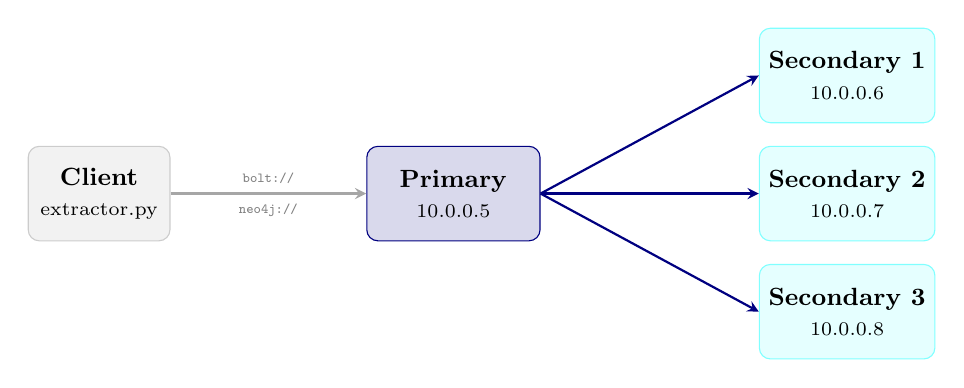
\begin{tikzpicture}[
    vm/.style={rectangle, draw=Navy, rounded corners,
               minimum width=2.2cm, minimum height=1.2cm,
               font=\small, align=center},
    primary/.style={vm, fill=Navy!15, draw=Navy},
    secondary/.style={vm, fill=Cyan!10, draw=Cyan!50},
    arrow/.style={->, thick, >=stealth, Navy},
    port/.style={font=\tiny, Gray}
  ]
    \node[primary] (p) at (-1, 0) {
      \textbf{Primary}\\
      \scriptsize 10.0.0.5
    };
    \node[secondary] (s1) at (4, 1.5) {
      \textbf{Secondary 1}\\
      \scriptsize 10.0.0.6
    };
    \node[secondary] (s2) at (4, 0) {
      \textbf{Secondary 2}\\
      \scriptsize 10.0.0.7
    };
    \node[secondary] (s3) at (4, -1.5) {
      \textbf{Secondary 3}\\
      \scriptsize 10.0.0.8
    };

    \draw[arrow] (p.east) -- (s1.west);
    \draw[arrow] (p.east) -- (s2.west);
    \draw[arrow] (p.east) -- (s3.west);

    \node[vm, fill=Gray!10, draw=Gray!40,
          minimum width=1.8cm] (client) at (-5.5, 0) {
      \textbf{Client}\\
      \scriptsize extractor.py
    };

    \draw[arrow, Gray!70] (client.east) --
      node[above, port]{\texttt{bolt://}}
      node[below, port]{\texttt{neo4j://}}
      (p.west);
  \end{tikzpicture}
  \end{center}

  \vspace{0.3em}

  \begin{columns}[t]
    \column{0.48\textwidth}
      \textcolor{Cyan}{\textbf{Primary}}\\[2pt]
      \small Scritture e consenso distribuito tramite protocollo Raft.

    \column{0.48\textwidth}
      \textcolor{Cyan}{\textbf{Secondary}}\\[2pt]
      \small Sola lettura: scalano le operazioni di estrazione dati.
  \end{columns}

\end{frame}



% decima slide
\begin{frame}{Pipeline sperimentale}

  Dal KG biomedico agli embedding, fino alla valutazione:
  una pipeline \hl{end-to-end} che collega infrastruttura
  e apprendimento automatico.

  \vspace{1em}

  \begin{center}
  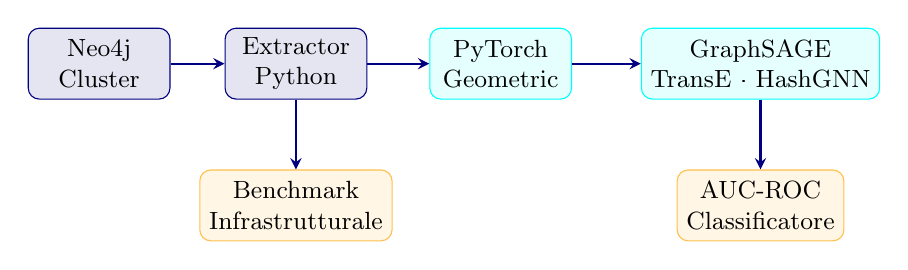
\begin{tikzpicture}[
    box/.style={rectangle, draw=Navy, rounded corners,
                minimum width=1.8cm, minimum height=0.9cm,
                font=\small, align=center, fill=Navy!10},
    cyanbox/.style={box, draw=Cyan, fill=Cyan!10},
    orangebox/.style={box, draw=Orange!70, fill=Orange!10},
    arrow/.style={->, thick, >=stealth, Navy}
  ]
    \node[box]      (kg)     at (0, 0)    {Neo4j\\Cluster};
    \node[box]      (ext)    at (2.5, 0)  {Extractor\\Python};
    \node[cyanbox]  (pyg)    at (5.1, 0)  {PyTorch\\Geometric};
    \node[cyanbox]  (models) at (8.4, 0)  {GraphSAGE\\TransE · HashGNN};
    \node[orangebox](eval)   at (8.4, -1.8) {AUC-ROC\\Classificatore};
    \node[orangebox](bench)  at (2.5, -1.8) {Benchmark\\Infrastrutturale};

    \draw[arrow] (kg)     -- (ext);
    \draw[arrow] (ext)    -- (pyg);
    \draw[arrow] (pyg)    -- (models);
    \draw[arrow] (models) -- (eval);
    \draw[arrow] (ext)    -- (bench);
  \end{tikzpicture}
  \end{center}

  \vspace{0.5em}

  \begin{center}
    \small\textcolor{Gray}{5 run indipendenti · 200 epoche ·
    test split 10\% · seed 42}
  \end{center}

\end{frame}



% undicesima slide
\begin{frame}{Benchmark infrastrutturale}

  Tempo di estrazione del sottografo Chemical$\to$Disease
  da Neo4j verso PyTorch Geometric al variare dei
  \hl{nodi attivi nel cluster}.

  \vspace{0.5em}

  \begin{columns}[c]
    \column{0.55\textwidth}
      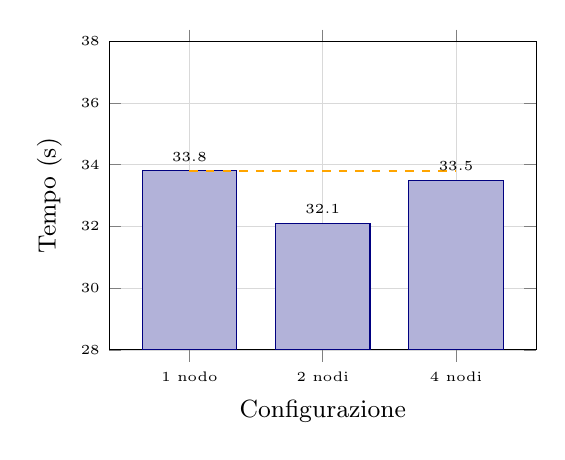
\begin{tikzpicture}
      \begin{axis}[
        ybar,
        bar width=1.2cm,
        width=7cm,
        height=5.5cm,
        xlabel={\small Configurazione},
        ylabel={\small Tempo (s)},
        symbolic x coords={1 nodo, 2 nodi, 4 nodi},
        xtick=data,
        ymin=28, ymax=38,
        ytick={28,30,32,34,36,38},
        tick label style={font=\tiny},
        label style={font=\small},
        enlarge x limits=0.3,
        grid=major,
        grid style={line width=0.2pt, draw=Gray!30},
        nodes near coords,
        every node near coord/.style={font=\tiny},
      ]
        \addplot[fill=Navy!30, draw=Navy] coordinates {
          (1 nodo, 33.8)
          (2 nodi, 32.1)
          (4 nodi, 33.5)
        };
        \draw[dashed, Orange, thick]
          (axis cs:1 nodo, 33.8) -- (axis cs:4 nodi, 33.8);
      \end{axis}
      \end{tikzpicture}

    \column{0.45\textwidth}
      \textcolor{Cyan}{\textbf{Risultato}}\\[6pt]
      \small I tempi sono sostanzialmente costanti tra le tre
      configurazioni. Il bottleneck è la \textbf{capacità di I/O
      sequenziale}, non la disponibilità di nodi.

      \vspace{0.8em}

      \textcolor{Cyan}{\textbf{Sweet spot}}\\[6pt]
      \small La configurazione a 2 nodi risulta leggermente
      più veloce: l'overhead di coordinamento supera il
      vantaggio con 4 nodi attivi.

  \end{columns}

\end{frame}



% dodicesima slide
\begin{frame}{Risultati: accuratezza}

  Tutti e tre i modelli raggiungono un'accuratezza elevata.
  \hl{GraphSAGE} domina con la deviazione standard più bassa,
  indicando alta stabilità statistica tra le run.

  \vspace{1.5em}

  \begin{columns}[t]
    \column{0.55\textwidth}
    \vfill
    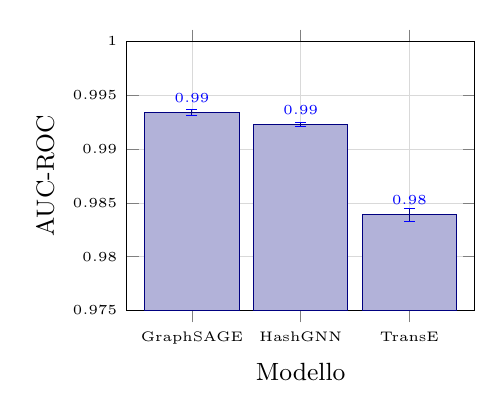
\begin{tikzpicture}
      \begin{axis}[
        ybar,
        bar width=1.2cm,
        width=6cm,
        height=5cm,
        xlabel={\small Modello},
        ylabel={\small AUC-ROC},
        symbolic x coords={GraphSAGE, HashGNN, TransE},
        xtick=data,
        ymin=0.975, ymax=1.0,
        ytick={0.975,0.980,0.985,0.990,0.995,1.0},
        yticklabel style={/pgf/number format/fixed,
                          /pgf/number format/precision=3,
                          font=\tiny},
        tick label style={font=\tiny},
        label style={font=\small},
        enlarge x limits=0.3,
        grid=major,
        grid style={line width=0.2pt, draw=Gray!30},
        error bars/y dir=both,
        error bars/y explicit,
        nodes near coords,
        every node near coord/.style={font=\tiny, anchor=south},
      ]
        \addplot+[fill=Navy!30, draw=Navy,
          error bars/.cd, y dir=both, y explicit] coordinates {
          (GraphSAGE, 0.9934) +- (0, 0.0003)
          (HashGNN,   0.9923) +- (0, 0.0002)
          (TransE,    0.9839) +- (0, 0.0006)
        };
      \end{axis}
      \end{tikzpicture}

    \column{0.45\textwidth}
    \vfill
      \kpi{0.9934}{GraphSAGE}
      \kpi{0.9923}{HashGNN}
      \kpi{0.9839}{TransE}

  \end{columns}

\end{frame}


% tredicesima slide
\begin{frame}{Risultati: efficienza e trade-off}

  \hl{TransE} è il più veloce di un margine significativo.
  GraphSAGE domina HashGNN in senso di Pareto: più accurato
  e più veloce contemporaneamente.

  \vspace{0.5em}

  \begin{columns}[t]
    \column{0.55\textwidth}
      \vfill
      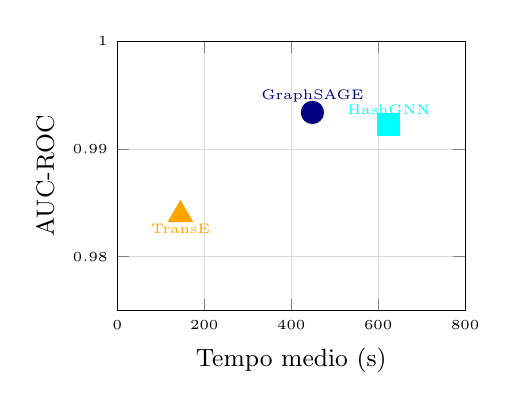
\begin{tikzpicture}
      \begin{axis}[
        width=6cm,
        height=5cm,
        xlabel={\small Tempo medio (s)},
        ylabel={\small AUC-ROC},
        xmin=0, xmax=800,
        ymin=0.975, ymax=1.0,
        yticklabel style={/pgf/number format/fixed,
                          /pgf/number format/precision=3,
                          font=\tiny},
        tick label style={font=\tiny},
        label style={font=\small},
        grid=both,
        grid style={line width=0.2pt, draw=Gray!30},
      ]
        \addplot[only marks, mark=*, mark size=4pt, Navy]
          coordinates {(448.7, 0.9934)};
        \addplot[only marks, mark=square*, mark size=4pt, Cyan]
          coordinates {(624.2, 0.9923)};
        \addplot[only marks, mark=triangle*, mark size=5pt, Orange]
          coordinates {(145.2, 0.9839)};
        \node[font=\tiny, Navy, anchor=south]
          at (axis cs:448.7, 0.9934) {GraphSAGE};
        \node[font=\tiny, Cyan, anchor=south]
          at (axis cs:624.2, 0.9923) {HashGNN};
        \node[font=\tiny, Orange, anchor=north]
          at (axis cs:145.2, 0.9839) {TransE};
      \end{axis}
      \end{tikzpicture}

    \column{0.45\textwidth}
      \vfill
      \kpi{145s}{TransE, il più veloce}
      \kpi{448s}{GraphSAGE}
      \kpi{624s}{HashGNN, il più lento}

  \end{columns}

\end{frame}



% quattordicesima slide
\begin{frame}{Verifica delle ipotesi}

  Le ipotesi iniziali sono state in parte \hl{smentite},
  con risultati scientificamente rilevanti in entrambi i casi.

  \vspace{0.8em}

  \begin{center}
  \begin{tabular}{lcc}
    \toprule
    \textbf{Ipotesi} & \textbf{Attesa} & \textbf{Risultato} \\
    \midrule
    Modello più accurato
      & HashGNN
      & \textcolor{Cyan}{GraphSAGE} \\[6pt]
    HashGNN supera GraphSAGE
      & \textcolor{Cyan}{Sì}
      & \textcolor{Orange}{No} \\[6pt]
    Speedup con 4 nodi
      & \textcolor{Cyan}{Sì}
      & \textcolor{Orange}{No} \\[6pt]
    TransE più efficiente
      & \textcolor{Cyan}{Sì}
      & \textcolor{Cyan}{Sì} \\
    \bottomrule
  \end{tabular}
  \end{center}

  \vspace{0.8em}

  \begin{center}
    \small\textcolor{Gray}{Un'ipotesi smentita con metodologia rigorosa
    ha lo stesso valore scientifico di un'ipotesi confermata.}
  \end{center}

\end{frame}



% quindicesima slide
\begin{frame}{Contributi e sviluppi futuri}

  \begin{columns}[t]
    \column{0.48\textwidth}
      \textcolor{Cyan}{\textbf{Contributi originali}}\\[6pt]
      \begin{itemize}
        \item Validazione empirica di tre paradigmi di embedding
          su un KG biomedico reale di scala massiva
        \item Profilazione end-to-end dell'overhead infrastrutturale
          da Graph DBMS distribuito a framework ML
        \item Infrastruttura riproducibile tramite
          \textit{Infrastructure as Code} con Ansible
      \end{itemize}

    \column{0.48\textwidth}
      \textcolor{Cyan}{\textbf{Sviluppi futuri}}\\[6pt]
      \begin{itemize}
        \item Estendere il confronto all'intero grafo eterogeneo
          con tutti i 410 tipi di relazione
        \item Aumentare il numero di epoche per HashGNN,
          penalizzato dalla convergenza più lenta
        \item Valutare l'impatto del cluster su carichi
          di lettura paralleli
        \item Integrare embedding nativi della libreria GDS
          di Neo4j
      \end{itemize}
  \end{columns}

\end{frame}



% sedicesima slide
\begin{frame}{Conclusioni}

  La GDS si conferma un paradigma efficace per l'analisi predittiva
  su KG biomedici di scala massiva, ma la scelta dell'algoritmo
  non è neutrale: ogni approccio riflette \hl{assunzioni architetturali}
  con impatti misurabili sulla qualità degli embedding.

  \vspace{1.5em}

  \begin{columns}[t]
    \column{0.33\textwidth}
      \textcolor{Cyan}{\textbf{GraphSAGE}}\\[4pt]
      \small Migliore accuratezza e convergenza rapida. Vince
      nonostante l'approccio omogeneo.

    \column{0.33\textwidth}
      \textcolor{Cyan}{\textbf{TransE}}\\[4pt]
      \small Vincitore dell'efficienza. Tre volte più veloce
      con un sacrificio minimo in accuratezza.

    \column{0.33\textwidth}
      \textcolor{Cyan}{\textbf{Infrastruttura}}\\[4pt]
      \small Il beneficio reale del cluster è la fault tolerance,
      non lo speedup su query sequenziali.
  \end{columns}

\end{frame}



% diciasettesima slide
\iniziofrontespizio
\begin{frame}[plain]
  \begin{tikzpicture}[remember picture, overlay]
    \node[anchor=north] at ([yshift=-0.8cm]current page.north)
      {
\includegraphics[height=1.8cm]{figures/logo_unime.png}};
    \node[anchor=center, text width=10cm, align=center]
      at (current page.center)
      {\Large\textcolor{white}{\textbf{Grazie per l'attenzione}}\\[12pt]
       \normalsize\textcolor{Gray}{Sandi Russo}\\[8pt]
       \small\textcolor{Gray}{Relatore: Prof. Antonio Celesti}\\[8pt]
       \small\textcolor{Gray}{Università degli Studi di Messina}\\[8pt]
       \small\textcolor{Gray}{A.A. 2025/2026}};
  \end{tikzpicture}
\end{frame}
\finefrontespizio



\end{document}